% !TEX program = lualatex
        
% IMPORTANT! In order for the document to compile, one needs to use XeLaTeX or LuaLaTeX as compiler. This can be done in  Overleaf by Menu -> Settings -> Compiler -> Choose XeLaTeX/LuaLaTeX
\documentclass[t,24pt,aspectratio=169]{beamer}

\usepackage{UAM}
\usepackage{multicol} % Package for multiple coloumns
\usepackage[style=authoryear]{biblatex}
\usepackage{listings}
\usepackage{xcolor}

\definecolor{codegreen}{rgb}{0,0.6,0}
\definecolor{codegray}{rgb}{0.5,0.5,0.5}
\definecolor{codepurple}{rgb}{0.58,0,0.82}
\definecolor{backcolour}{rgb}{0.95,0.95,0.92}

\lstset{
	backgroundcolor=\color{backcolour},
	commentstyle=\color{codegreen},
	keywordstyle=\color{magenta},
	numberstyle=\tiny\color{codegray},
	stringstyle=\color{codepurple},
	basicstyle=\ttfamily\footnotesize,
	breaklines=true,
	frame=single,
	showstringspaces=false
}

%\usepackage{minted}
% lualatex -shell-escape -synctex=1 -interaction=nonstopmode archivo.tex

% \toplinje{Text at top} % The text at top. Remove the command if no text is desired


\addbibresource{references.bib}
\begin{document}

% The first slide. One can for instance change the main title, the subtitle, speaker, KU-unit, date and backgroundimage
{
\setbeamertemplate{background}{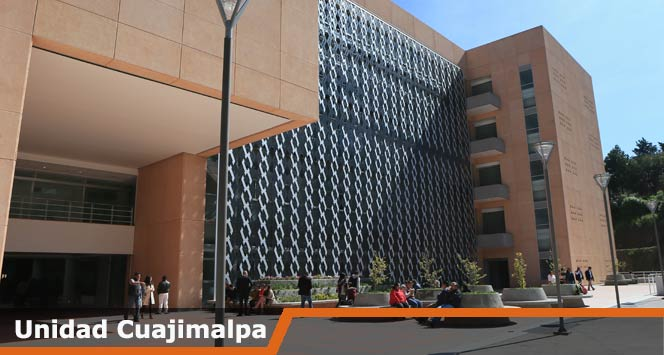
\includegraphics[width=\paperwidth,height=\paperheight]{uam/cua_05.jpg}}
\begin{frame}
    \begin{textblock*}{\textwidth}(0.53\textwidth,0.1\textheight)
        \begin{beamercolorbox}[wd=8.5cm,ht=7.3cm,sep=0.5cm]{hvidbox}
            \fontsize{5}{10}\fontfamily{ptm}\selectfont \textls[200]{UNIVERSIDAD AUTÓNOMA METROPOLITANA}
            \noindent\textcolor{KUrod}{\rule{6.8cm}{0.4pt}}
        \end{beamercolorbox}
    \end{textblock*}
    \begin{textblock*}{\textwidth}(0.53\textwidth,0.1\textheight)
        \begin{beamercolorbox}[wd=8.5cm,sep=0.5cm]{hvidbox}
                \Huge \textcolor{KUrod}{Integración de sistemas}
                \vspace{0.5cm}
                \par
                \Large SOAP hoy...

                \vspace{0.5cm}
                \par
                \normalsize Juan Alvarado
        \end{beamercolorbox}
    \end{textblock*}
    \begin{textblock}{1}(14.5,11.38)
        % \includegraphics[width=1cm]{KU/KU-logo.png}
    \end{textblock}
\end{frame}
}


        %%%%%%%%%%%%%%%%%%%%%%%%%%%%%%%%%%%%%%%
	\begin{frame}[fragile, hvid]
		\frametitle{Sectores donde SOAP sigue vigente}
			\vfill
			\centering
			\Huge{Sectores donde SOAP sigue vigente}
			\vfill
	\end{frame}
%%%%%%%%%%%%%%%%%%%%%%%%%%%%%%%%%%%%%%%


%%%%%%%%%%%%%%%%%%%%%%%%%%%%%%%%%%%%%%%
	\begin{frame}[fragile, hvid]
		\frametitle{Sectores donde SOAP sigue vigente}
			\vfill
\begin{multicols}{2} 

Aunque muchas integraciones nuevas usan APIs REST o variantes modernas, SOAP sigue siendo relevante en sectores con fuertes requisitos regulatorios y de seguridad.
\\~\\
\columnbreak
\centering

\includegraphics[width=6.6cm,height=5.9cm,keepaspectratio]{img/pexels-lukas-574069.jpg}
\end{multicols}
			\vfill
	\end{frame}
%%%%%%%%%%%%%%%%%%%%%%%%%%%%%%%%%%%%%%%


%%%%%%%%%%%%%%%%%%%%%%%%%%%%%%%%%%%%%%%
	\begin{frame}[fragile, hvid]
		\frametitle{Sectores donde SOAP sigue vigente}
			\vfill
\begin{multicols}{2} 

En banca, numerosos servicios de pago, compensación y reporteo se apoyan en servicios web SOAP por sus contratos formales, soporte para WS-Security y herramientas maduras.
\\~\\
\columnbreak
\centering

\includegraphics[width=6.6cm,height=5.9cm,keepaspectratio]{img/warning-g9e7961896_640.png}
\end{multicols}
			\vfill
	\end{frame}
%%%%%%%%%%%%%%%%%%%%%%%%%%%%%%%%%%%%%%%


%%%%%%%%%%%%%%%%%%%%%%%%%%%%%%%%%%%%%%%
	\begin{frame}[fragile, hvid]
		\frametitle{Sectores donde SOAP sigue vigente}
			\vfill
En gobierno, muchas plataformas de interoperabilidad entre dependencias se estandarizaron hace años en torno a SOAP, y migrar toda esa infraestructura es costoso y arriesgado.
\\~\\
			\vfill
	\end{frame}
%%%%%%%%%%%%%%%%%%%%%%%%%%%%%%%%%%%%%%%


%%%%%%%%%%%%%%%%%%%%%%%%%%%%%%%%%%%%%%%
	\begin{frame}[fragile, hvid]
		\frametitle{Sectores donde SOAP sigue vigente}
			\vfill
\begin{multicols}{2} 

En salud, estándares como HL7 y ciertas pasarelas de intercambio clínico han utilizado SOAP y WS- para garantizar trazabilidad, autenticación y cifrado robusto.
\\~\\
\columnbreak
\centering

\includegraphics[width=6.6cm,height=5.9cm,keepaspectratio]{img/Question mark.jpg}
\end{multicols}
			\vfill
	\end{frame}
%%%%%%%%%%%%%%%%%%%%%%%%%%%%%%%%%%%%%%%


%%%%%%%%%%%%%%%%%%%%%%%%%%%%%%%%%%%%%%%
	\begin{frame}[fragile, hvid]
		\frametitle{APIs modernas: REST y más allá}
			\vfill
			\centering
			\Huge{APIs modernas: REST y más allá}
			\vfill
	\end{frame}
%%%%%%%%%%%%%%%%%%%%%%%%%%%%%%%%%%%%%%%


%%%%%%%%%%%%%%%%%%%%%%%%%%%%%%%%%%%%%%%
	\begin{frame}[fragile, hvid]
		\frametitle{APIs modernas: REST y más allá}
			\vfill
Las APIs modernas suelen exponer recursos a través de HTTP usando REST y formatos ligeros como JSON, lo que simplifica el consumo desde navegadores, apps móviles y microservicios.
\\~\\
			\vfill
	\end{frame}
%%%%%%%%%%%%%%%%%%%%%%%%%%%%%%%%%%%%%%%


%%%%%%%%%%%%%%%%%%%%%%%%%%%%%%%%%%%%%%%
	\begin{frame}[fragile, hvid]
		\frametitle{APIs modernas: REST y más allá}
			\vfill
Estas APIs favorecen ciclos de desarrollo rápidos, menores dependencias de herramientas específicas y una curva de aprendizaje más suave para desarrolladores.
\\~\\
Nuevos enfoques como GraphQL, gRPC o arquitecturas basadas en eventos amplían el repertorio.
\\~\\
			\vfill
	\end{frame}
%%%%%%%%%%%%%%%%%%%%%%%%%%%%%%%%%%%%%%%


%%%%%%%%%%%%%%%%%%%%%%%%%%%%%%%%%%%%%%%
	\begin{frame}[fragile, hvid]
		\frametitle{APIs modernas: REST y más allá}
			\vfill
No obstante, es importante entender que en la práctica conviven servicios SOAP heredados con APIs modernas, y muchos proyectos requieren integrar ambos mundos.
\\~\\
			\vfill
	\end{frame}
%%%%%%%%%%%%%%%%%%%%%%%%%%%%%%%%%%%%%%%


%%%%%%%%%%%%%%%%%%%%%%%%%%%%%%%%%%%%%%%
	\begin{frame}[fragile, hvid]
		\frametitle{Cuándo SOAP sigue siendo una opción razonable}
			\vfill
			\centering
			\Huge{Cuándo SOAP sigue siendo una opción razonable}
			\vfill
	\end{frame}
%%%%%%%%%%%%%%%%%%%%%%%%%%%%%%%%%%%%%%%


%%%%%%%%%%%%%%%%%%%%%%%%%%%%%%%%%%%%%%%
	\begin{frame}[fragile, hvid]
		\frametitle{Cuándo SOAP sigue siendo una opción razonable}
			\vfill
SOAP puede seguir siendo una opción razonable cuando se necesitan contratos \textbf{altamente estructurados}, \textbf{transacciones distribuidas complejas o cumplimiento de estándares existentes} que ya asumen la pila SOAP.
\\~\\
			\vfill
	\end{frame}
%%%%%%%%%%%%%%%%%%%%%%%%%%%%%%%%%%%%%%%


%%%%%%%%%%%%%%%%%%%%%%%%%%%%%%%%%%%%%%%
	\begin{frame}[fragile, hvid]
		\frametitle{Cuándo SOAP sigue siendo una opción razonable}
			\vfill
\begin{multicols}{2} 

Esto es frecuente en integraciones \textbf{interorganizacionales} donde el contrato se negocia una vez y debe mantenerse \textbf{estable durante muchos años}.
\\~\\
\columnbreak
\centering

\includegraphics[width=6.6cm,height=5.9cm,keepaspectratio]{img/pexels-sora-shimazaki-5935755.jpg}
\end{multicols}
			\vfill
	\end{frame}
%%%%%%%%%%%%%%%%%%%%%%%%%%%%%%%%%%%%%%%


%%%%%%%%%%%%%%%%%%%%%%%%%%%%%%%%%%%%%%%
	\begin{frame}[fragile, hvid]
		\frametitle{Cuándo SOAP sigue siendo una opción razonable}
			\vfill
\begin{multicols}{2} 

También puede ser más sencillo consumir un servicio SOAP existente que reescribirlo en REST, sobre todo si el proveedor solo ofrece WSDL y documentación WS-.
\\~\\
\columnbreak
\centering

\includegraphics[width=6.6cm,height=5.9cm,keepaspectratio]{img/pexels-fauxels-3182812.jpg}
\end{multicols}
			\vfill
	\end{frame}
%%%%%%%%%%%%%%%%%%%%%%%%%%%%%%%%%%%%%%%


%%%%%%%%%%%%%%%%%%%%%%%%%%%%%%%%%%%%%%%
	\begin{frame}[fragile, hvid]
		\frametitle{Cuándo SOAP sigue siendo una opción razonable}
			\vfill
El reto para el arquitecto es decidir cuándo convivir con SOAP y encapsularlo, y cuándo impulsar una migración hacia APIs más ligeras.
\\~\\
			\vfill
	\end{frame}
%%%%%%%%%%%%%%%%%%%%%%%%%%%%%%%%%%%%%%%


%%%%%%%%%%%%%%%%%%%%%%%%%%%%%%%%%%%%%%%
	\begin{frame}[fragile, hvid]
		\frametitle{Práctica}
			\vfill
			\centering
			\Huge{Práctica}
			\vfill
	\end{frame}
%%%%%%%%%%%%%%%%%%%%%%%%%%%%%%%%%%%%%%%


%%%%%%%%%%%%%%%%%%%%%%%%%%%%%%%%%%%%%%%
	\begin{frame}[fragile, hvid]
		\frametitle{Práctica}
			\vfill
\textbf{Explorando un WSDL y comparándolo con una API REST}
\\~\\
En esta práctica inspeccionarán un archivo WSDL y lo compararán conceptualmente con la documentación de una API REST, identificando elementos de contrato en ambos casos.
\\~\\
			\vfill
	\end{frame}
%%%%%%%%%%%%%%%%%%%%%%%%%%%%%%%%%%%%%%%


{
	\setbeamertemplate{background}{
\includegraphics[width=\paperwidth,height=\paperheight]{uam/cua_01.jpg}}
	\begin{frame}[billede]
		\begin{textblock*}{\textwidth}(0\textwidth,0.77\textheight)
			\begin{beamercolorbox}[wd=7.8cm,sep=0.3cm]{rodbox}
				{\huge ¡Gracias!}
			\end{beamercolorbox}
		\end{textblock*}
	\end{frame}
}

%%%%% THIS IS THE BLOCK OF REFERENCES 

% \begin{frame}[hvid, allowframebreaks]
	% \frametitle{Referencias}
	% \printbibliography
	
	% \end{frame}


%%%%%% END OF THE BLOCK OF REFERENCES

\end{document}
